\section{Conclusion}
\subsection{Results}
% \begin{frame}{Results System Design}
%     \centering
%     \vfill
%     \begin{tabular}{r | l}
%         Successes & Improvements to make \\
%         \hline
%         the glove is non-obstructive & robustness \\
%         performance good enough for prototype & generalization to different hand types \\
%         architecture proved suitable & one piece glove \\
%     \end{tabular}
% \end{frame}

\begin{frame}{Results System Design}
    \begin{block}{Goal (Reminder)}
        Design a system for recording characteristic hand movements of typing
        and the corresponding input.
    \end{block}
    \pause
    \vfill\null
    \begin{columns}[T]
        \begin{column}{0.5\textwidth}
            \textbf{Successes}
            \begin{itemize}
                \item the architecture proved suitable
                \item the glove is non-obstructive
                \item performance is good enough for a prototype
            \end{itemize}
        \end{column}
        \begin{column}{0.5\textwidth}
            \textbf{Improvements}
            \begin{itemize}
                \item gyro clipping
                \item single robust glove
                \item generalization to different hand types
            \end{itemize}
        \end{column}
    \end{columns}
\end{frame}

\begin{frame}{Results Machine Learning}
    \begin{block}{Goal (Reminder)}
        Define an approach for utilizing machine learning to map the recorded
        data back to the keyboard input.
    \end{block}
    \pause
    \vfill\null
    \begin{columns}[T]
        \begin{column}{0.5\textwidth}
            \textbf{Successes}
            \begin{itemize}
                \item slow typing can be distinguished
                \item preprocessing helps the learning progress
                \item CNNs can distinguish between different keys
            \end{itemize}
        \end{column}
        \begin{column}{0.5\textwidth}
            \textbf{Improvements}
            \begin{itemize}
                \item better accuracy
                \item reduce delay
                \item detect holding a key
                \item detect different modes $\rightarrow$(non-)writing position
            \end{itemize}
        \end{column}
    \end{columns}

    \notes{
        \item fscore, recall, precision
        \item delay
            \begin{itemize}
                \item keystroke in middle
                \item 8 timesteps before and after
            \end{itemize}
        \item learn on more data (accel, gyro..)
            \begin{itemize}
                \item learn more about hand position not only orientation
            \end{itemize}
    }
\end{frame}
% \begin{frame}{Results}{Successes System Design}
%     \begin{itemize}
%     \end{itemize}
% \end{frame}
% \begin{frame}{Results}{Successes Machine Learning}
%         \begin{itemize}
%         \end{itemize}
% \end{frame}
% \begin{frame}{Results}{Failures}
%     \begin{itemize}
%         \item RNN did not work
%         \begin{itemize}
%             \item therefore we did preprocessing and looked at the structure of our data
%         \end{itemize}
%         \item huge delays
%         \begin{itemize}
%             \item can be reduced by using another time step window around keypress event
%         \end{itemize}
%         \item cannot detect holding key
%         \begin{itemize}
%             \item use all imu data to get a better understanding of actual hand position
%             \item learn key releases
%         \end{itemize}
%     \end{itemize}
% \end{frame}

\subsection{Outlook}
\begin{frame}{Outlook}
    \begin{block}{Goal (Reminder)}
        Evaluate the quality of such mapping and discuss whether this principle
        could be turned into a working keyboard alternative.
    \end{block}
    \pause
    \vfill\null
    \begin{itemize}
        \item reduce delay, remove lookaheads
        \item increase prediction quality
        \item two hands
        \item generalize glove \& model
        \item implement online learning
        \item better hand pose reconstruction for more use cases
        % \item publish schematics and instructions for building the glove
    \end{itemize}
\end{frame}

\appendix
\begin{frame}[allowframebreaks]{References}
    \renewcommand*{\bibfont}{\scriptsize}
    \printbibliography
\end{frame}

\begin{frame}[plain]
   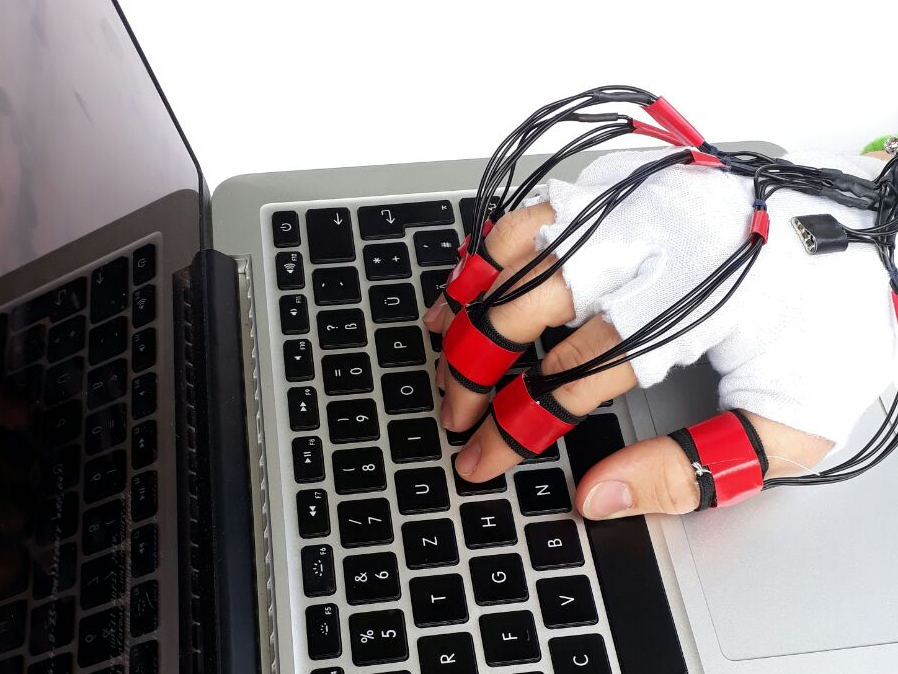
\includegraphics[width=0.9\textwidth]{../common/images/glove-live}
\end{frame}


\begin{frame}[plain]
   \begin{figure}
       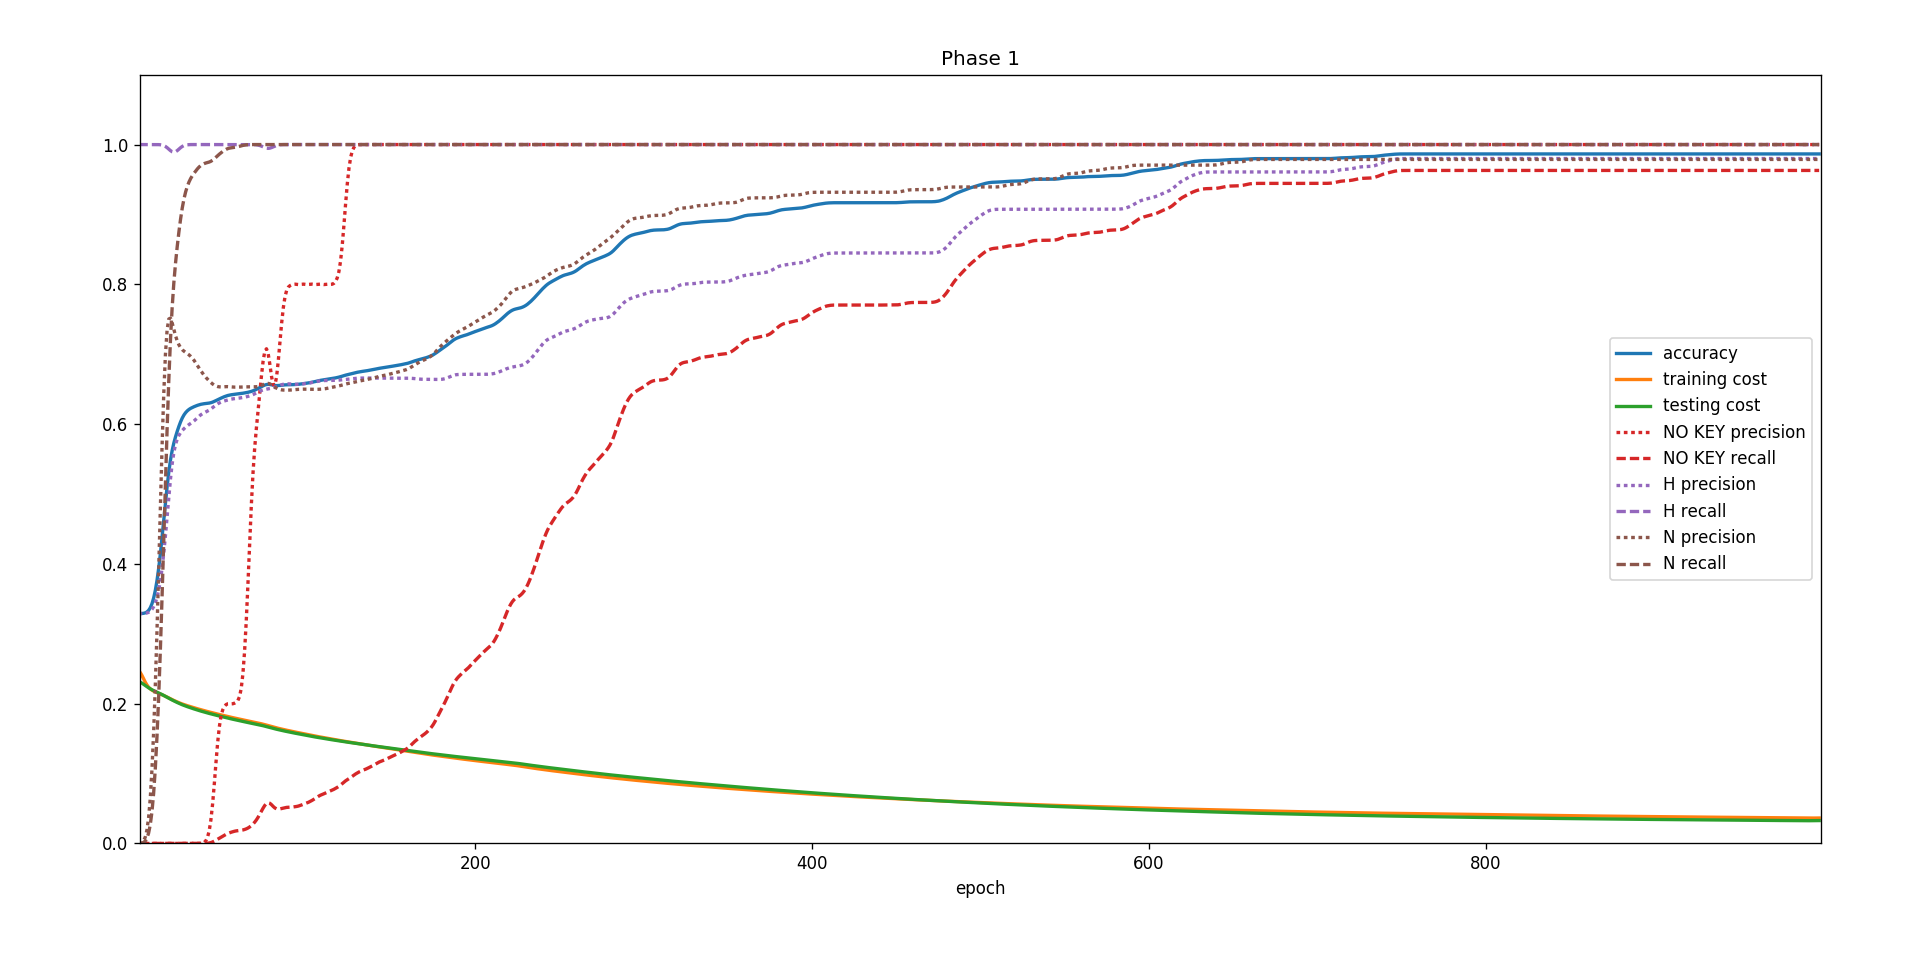
\includegraphics[width=\textwidth]{../common/images/phase-1-detailed}
       \label{fig:phase22}
       \caption{Performance metrics of phase 1, including per key precision and recall}
   \end{figure}
\end{frame}

